\documentclass[dvipdfmx]{article}

\usepackage[a4paper, margin=2cm]{geometry}
\usepackage[dvipdfmx]{graphicx}

\title{Low Power Coding with Balanced Ternary for Communications using spread spectrum}
\author{Hirano Takeshi \thanks{hyranno4pub@gmail.com http://uncotechhack.net}}
\date{2020/04/04}

\begin{document}

\maketitle

\begin{abstract}
Coding with balanced ternary for communications using spread spectrum is proposed in this article.
The proposed code with large number of codewords can achieve lower power cost than binary code.
The proposed code with long spreading code even can achieve larger line rate than binary code.
\end{abstract}


\section{Power Cost of Binary and Balanced Ternary}
Like as binary represents numbers with symbols $\{ 0,1\}$ or $\{ \bar{1}, 1\}$,
 balanced ternary represents numbers with symbols $\{ \bar{1}, 0, 1\}$.

According to Hartley,
 if transmitter has amplitude range $\left[ -A, ... , +A \right]$ volts and the precision of the receiver is $\Delta V$ volts,
 the maximum number of distinguishable pulse levels $N$ has relation represented as equation\ref{eq:hartley}.

\begin{eqnarray}
	N &=& 1+\frac{A}{\Delta V} \nonumber \\
	A &=& \Delta V(N-1)
	\label{eq:hartley}
\end{eqnarray}

The amplitude of each symbol can be represented as
 $\{-\Delta V, +\Delta V \}$ for binary and
 $\{-2\Delta V, 0, +2\Delta V \}$ for balanced ternary.
With power cost $P_{2}$ of a binary symbol, power cost of ternary symbol is represented as $\{ 4P_{2}, 0, 4P_{2} \}$.
The power cost is different with the symbol in balanced ternary.
Coding with less symbol $1$ and $\bar{1}$, the power cost of the code can be decreased.


\section{Low Power Coding}
I propose variable-length code in this article.
Padding with $0$ will convert it to fixed-length code.
Communication is assumed to use spread spectrum.
A single spreading code is used, and it is binary because $0$ does not contribute to voltage level.

Code with minimum number of symbol $1$ and $\bar{1}$ can be represented as
 $\{ 1, \bar{1}, 01, 0\bar{1}, 001, 00\bar{1}, 0001, 000\bar{1}, ... \}$.
With spreading code $s$, the code is
 $\{ s, \bar{s}, 0s, 0\bar{s}, 00s, 00\bar{s}, 000s, 000\bar{s}, ... \}$.
Each codeword can be send with the power cost of a single spreading code.
Because $0$ cannot be spreaded,
 time length of the symbol $0$ can be shortened from the time length of the symbol $s$.
In other words, the codeword consists of
 the sign of the spreading code and
 the period between the spreading code and the former spreading code.


\section{Characteristics}
In this section, I reveal the characteristics of the proposed code comparing to the binary code.

Each codeword appears in equal possibility.
Equations uses
 $T_{0}$ as the time length of a symbol $0$,
 $T_{s}$ as the time length of the spreading code,
 $N_{c}$ as the number of multiple access,
 $N_{w}$ as the number of the codewords,
 $N_{0}$ as the number of the levels of the continuous time length sending $0$,
 and $H$ as the mean information content of the codewords.
$N_{0}$ is represented as equation\ref{eq:N0}.
$H$ is represented as equation\ref{eq:H}.

\begin{eqnarray}
	N_{0} = \frac{N_{w}}{2}
	\label{eq:N0}
\end{eqnarray}

\begin{eqnarray}
    H &=& \log_2(N_{w}) \nonumber \\
      &=& \log_2(2N_{0})
    \label{eq:H}
\end{eqnarray}

For the proposed code, equations\ref{eq:Pa3} to \ref{eq:R3} reapresent
 $P_{a3}$ as the power cost of a codeword,
 $T_{a3}$ as the average time length of codewords,
 $P_{h3}$ as the mean power cost per information content,
 and $R_{3}$ as the line rate.

\begin{eqnarray}
    P_{a3} = 4P_{2}
    \label{eq:Pa3}
\end{eqnarray}

\begin{eqnarray}
    T_{a3} = T_{s} + \frac{T_{0}(N_{0}-1)}{2}
    \label{eq:Ta3}
\end{eqnarray}

\begin{eqnarray}
    P_{h3} &=& \frac{P_{a3}}{H} \nonumber \\
    	&=& \frac{4P_{2}}{\log_2(N_{w})}
    \label{eq:Ph3}
\end{eqnarray}

\begin{eqnarray}
    R_{3} &=& N_{c} \frac{H}{T_{a3}} \nonumber \\
      &=& \frac{ N_{c}\log_2(2N_{0}) }{ T_{s}+\frac{T_{0}(N_{0}-1)}{2} }
    \label{eq:R3}
\end{eqnarray}

For the binary code, equations\ref{eq:Pa2} to \ref{eq:R2} reapresent
 $P_{a2}$ as the power cost of a codeword,
 $T_{a2}$ as the average time length of codewords,
 $P_{h2}$ as the mean power cost per information content,
 and $R_{2}$ as the line rate.

\begin{eqnarray}
    P_{a2} = P_{2} \log_2(N_{w})
    \label{eq:Pa2}
\end{eqnarray}

\begin{eqnarray}
    T_{a2} = T_{s} \log_2(N_{w})
    \label{eq:Ta2}
\end{eqnarray}

\begin{eqnarray}
    P_{h2} &=& \frac{P_{a2}}{H} \nonumber \\
      &=& P_{2}
    \label{eq:Ph2}
\end{eqnarray}

\begin{eqnarray}
    R_{2} &=& N_{c} \frac{H}{T_{a2}} \nonumber \\
      &=& \frac{N_{c}}{T_{s}}
    \label{eq:R2}
\end{eqnarray}


$P_{h3}/P_{h2}$, the power cost ratio of the proposed code to the binary code, is represented as equation\ref{eq:pratio}.
The condition to achieve $P_{h3}/P_{h2} < 1$ is represented as equation\ref{eq:pratiocond}.
Figure\ref{fig:pratio} shows equation\ref{eq:pratio}.
You can see that the power cost ratio get smaller with the larger number of codewords.

\begin{eqnarray}
    \frac{P_{h3}}{P_{h2}} = \frac{4}{\log_2(N_{w})}
    \label{eq:pratio}
\end{eqnarray}

\begin{eqnarray}
    N_{w}>16
    \label{eq:pratiocond}
\end{eqnarray}

\begin{figure}[htbp]
  \begin{center}
    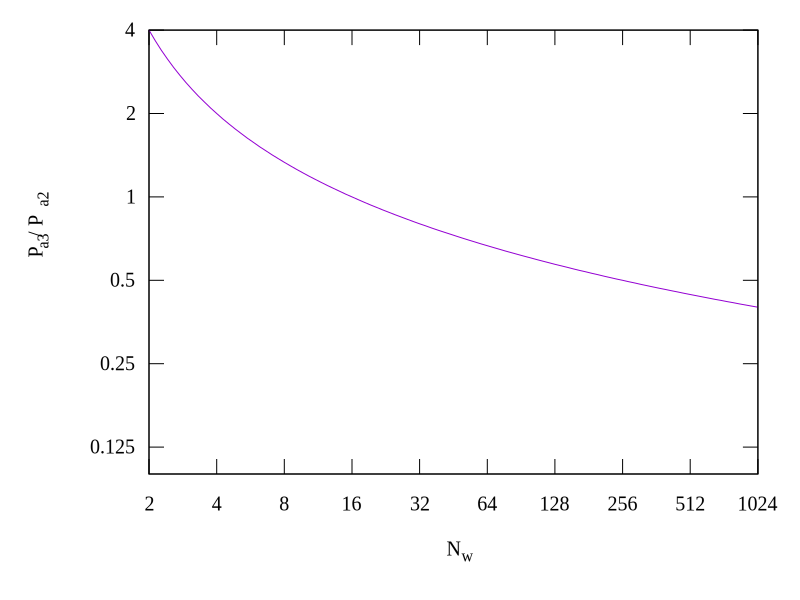
\includegraphics[clip, width=0.9\hsize, bb=0 0 800 600]{./resources/P.svg}
    \caption{power cost ratio of the proposed code to the binary code}
    \label{fig:pratio}
  \end{center}
\end{figure}
\, \newline

$R_{3}/R_{2}$, the line rate ratio of the proposed code to the binary code, is represented as equation\ref{eq:rratio}.
The condition to achieve $R_{3}/R_{2} > 1$ is represented as equation\ref{eq:rratiocond}.
Figure\ref{fig:rratio} shows equation\ref{eq:rratio}.
In Figure\ref{fig:rratio}, horizontal axis shows $N_{w}$, vertical axis shows $T_{0}/T_{s}$, and color bar shows $R_{3}/R_{2}$.
You can see that the line rate ratio get larger with the smaller $T_{0}/T_{s}$,
 or namely the larger length of the spreading code.

\begin{eqnarray}
    \frac{R_{3}}{R_{2}} &=& \frac{ T_{s}\log_2(2N_{0}) }{ T_{s}+\frac{T_{0}(N_{0}-1)}{2} } \nonumber \\
    	&=& \frac{ \log_2(N_{w}) }{ 1+\frac{T_{0}}{T_{s}} \frac{N_{w}-2}{4} }
    \label{eq:rratio}
\end{eqnarray}

\begin{eqnarray}
    4\frac{\log_2(N_{w})-1}{N_{w}-2} > \frac{T_{0}}{T_{s}}
    \label{eq:rratiocond}
\end{eqnarray}

\begin{figure}[htbp]
  \begin{center}
    \includegraphics[clip, width=0.9\hsize, bb=0 0 800 600]{./resources/R.svg}
    \caption{line rate ratio of the proposed code to the binary code}
    \label{fig:rratio}
  \end{center}
\end{figure}
\, \newline

It is still unclear that the proposed code fits in Shannon-Hartley theorem.
In Hartley's law, information content of a pulse is
 logarithm of the number of distinguishable pulse levels.
But in proposed code, information content depends on
 the number of distinguishable time period levels between pulses rather than pulse levels.

 
\section{Conclusion}
Coding with balanced ternary for communications using spread spectrum is proposed in this article.
The proposed code with large number of codewords can achieve lower power cost than binary code.
The proposed code with long spreading code even can achieve larger line rate than binary code.



\end{document}